% This is the Reed College LaTeX thesis template. Most of the work 
% for the document class was done by Sam Noble (SN), as well as this
% template. Later comments etc. by Ben Salzberg (BTS). Additional
% restructuring and APA support by Jess Youngberg (JY).
% Your comments and suggestions are more than welcome; please email
% them to cus@reed.edu
%
% See http://web.reed.edu/cis/help/latex.html for help. There are a 
% great bunch of help pages there, with notes on
% getting started, bibtex, etc. Go there and read it if you're not
% already familiar with LaTeX.
%
% Any line that starts with a percent symbol is a comment. 
% They won't show up in the document, and are useful for notes 
% to yourself and explaining commands. 
% Commenting also removes a line from the document; 
% very handy for troubleshooting problems. -BTS

% As far as I know, this follows the requirements laid out in 
% the 2002-2003 Senior Handbook. Ask a librarian to check the 
% document before binding. -SN

%%
%% Preamble
%%
% \documentclass{<something>} must begin each LaTeX document
\documentclass[12pt,twoside]{reedthesis}
% Packages are extensions to the basic LaTeX functions. Whatever you
% want to typeset, there is probably a package out there for it.
% Chemistry (chemtex), screenplays, you name it.
% Check out CTAN to see: http://www.ctan.org/
%%
\usepackage{graphicx,latexsym} 
\usepackage{amssymb,amsthm,amsmath}
\usepackage{longtable,booktabs,setspace} 
\usepackage{chemarr} %% Useful for one reaction arrow, useless if you're not a chem major
\usepackage[hyphens]{url}
\usepackage{rotating}
\usepackage{natbib}
\usepackage{ifthen}
\usepackage{color}
\usepackage[export]{adjustbox}[2011/08/13]
\graphicspath{{./Figs/}} % Set graphics path
% Comment out the natbib line above and uncomment the following two lines to use the new 
% biblatex-chicago style, for Chicago A. Also make some changes at the end where the 
% bibliography is included. 
%\usepackage{biblatex-chicago}
%\bibliography{thesis}

% \usepackage{times} % other fonts are available like times, bookman, charter, palatino


%%%% REFERENCES %%%%%
\newcommand{\rf}     [1] {~\cite{#1}}
\newcommand{\refref} [1] {ref.~\cite{#1}}
\newcommand{\refRef} [1] {Ref.~\cite{#1}}
\newcommand{\refrefs}[1] {refs.~\cite{#1}}
\newcommand{\refRefs}[1] {Refs.~\cite{#1}}
\newcommand{\refeq}  [1] {Eq.~(\ref{#1})}
\newcommand{\refeqs} [2]{Eqs.~\ref{#1} and \ref{#2}}
\newcommand{\refFig} [1] {Fig.~\ref{#1}}
\newcommand{\refFigs} [2] {Figs.~\ref{#1} and~\ref{#2}}
\newcommand{\reftab} [1] {Table~\ref{#1}}
\newcommand{\refTab} [1] {Table~\ref{#1}}
\newcommand{\reftabs}[2] {tables~\ref{#1} and~\ref{#2}}
\newcommand{\refsect}[1] {Section~\ref{#1}}
\newcommand{\refsects}[2] {Sections~\ref{#1} and \ref{#2}}
\newcommand{\refSect}[1] {Section~\ref{#1}}
\newcommand{\refSects}[2] {Sects.~\ref{#1} and \ref{#2}}
\newcommand{\refsecttosect}[2] {Sects.~\ref{#1} to~\ref{#2}}
\newcommand{\refappe}[1] {appendix~\ref{#1}}
\newcommand{\refappes}[2] {appendices~\ref{#1} and~\ref{#2}}
\newcommand{\refAppe}[1] {Appendix~\ref{#1}}
\newcommand{\refChapter}[1]{Chapter~\ref{#1}}
\newcommand{\refChapt}[1]{Chapt.~\ref{#1}}
\newcommand{\ignore}[1]{}
\newcommand{\nobibentry}[1]{{\let\nocite\ignore\bibentry{#1}}}
\newcommand{\bibfnamefont}[1]{#1}
\newcommand{\bibnamefont}[1]{#1}


%%%% SYMBOLS %%%%
\newcommand{\ReN}{\ensuremath{Re}} % Reynolds number

%%%% ABBREVIATIONS %%%%%
\newcommand{\etc}{{etc.}}       % APS
\newcommand{\etal}{{\em et al.}}    % etal in italics, APS too
\newcommand{\ie}{{i.e.}}        % APS
\newcommand{\cf}{{\em cf.\ }}     % APS
\newcommand{\eg}{{e.g.\ }}        % APS, OUP, hard space '\eg\ NextWord'

%%%%% EDITING COMMANDS %%%%%
\newcommand{\DB}[2]{$\footnotemark\footnotetext{DB #1: {\color{red}#2}}$} %date, comment
\newcommand{\DBedit}[1]{{\color{red}#1}}
\newcommand{\MC}[2]{$\footnotemark\footnotetext{DB #1: {\color{green}#2}}$} %date, comment
\newcommand{\MCedit}[1]{{\color{green}#1}}
 % Load thesis specific macros

\title{On Bouncing Oil Drops}
\author{Miguel B. Conner}
% The month and year that you submit your FINAL draft TO THE LIBRARY (May or December)
\date{May 2015}
\division{Mathematics and Natural Sciences}
\advisor{Daniel Borrero}
%If you have two advisors for some reason, you can use the following
%\altadvisor{Your Other Advisor}
%%% Remember to use the correct department!
\department{Physics}
% if you're writing a thesis in an interdisciplinary major,
% uncomment the line below and change the text as appropriate.
% check the Senior Handbook if unsure.
%\thedivisionof{The Established Interdisciplinary Committee for}
% if you want the approval page to say "Approved for the Committee",
% uncomment the next line
%\approvedforthe{Committee}

\setlength{\parskip}{0pt}
%%
%% End Preamble
%%
%% The fun begins:
\begin{document}

  \maketitle
  \frontmatter % this stuff will be roman-numbered
  \pagestyle{empty} % this removes page numbers from the frontmatter

% Acknowledgements (Acceptable American spelling) are optional
% So are Acknowledgments (proper English spelling)
%	% Acknowledgements (Acceptable American spelling) are optional
% So are Acknowledgments (proper English spelling)
    \chapter*{Acknowledgements}
	I want to thank a few people.
	
	%Help with thesis
	%Daniel, Jay, Bob. Kai, Lily, jack for reading drafts. daniel
	
	%Physics profs
	%Daniel, Darrell, Nelia, johnny, Joel, Lucas
	
	%Other profs
	% Albert, Libby, Alan (sp?), 
	
	% Parents
	
	% Kai
	
	% Lily and Clops
	
	

% The preface is optional
% To remove it, comment it out or delete it.
%	% The preface is optional
% To remove it, comment it out or delete it.
    \chapter*{Preface}
	This is an example of a thesis setup to use the reed thesis document class.

%  \tableofcontents
% if you want a list of tables, optional
%  \listoftables
% if you want a list of figures, also optional
%  \listoffigures
		
% The abstract is not required if you're writing a creative thesis (but aren't they all?)
% If your abstract is longer than a page, there may be a formatting issue.
%	% The abstract is not required if you're writing a creative thesis (but aren't they all?)
% If your abstract is longer than a page, there may be a formatting issue.
    \chapter*{Abstract}
	In 2005 Yves Couder's group discovered that and oil droplet placed on a vibrating bath of the same oil would bounce along the surface of the oil indefinitely, propelled by the waves it created \rf{Couder2005a}. This ``walker" exhibits many behaviors analogous to those observed in quantum systems, such as single particle double slit diffraction \rf{double-slit}, quantized orbits \rf{Oza2014}, and among others \rf{pilot-wave}, tunneling \rf{tunneling}. Tunneling occurs when a droplet interacts with a subsurface barrier; the droplet either passes over or reflects off of the barrier. In experiments described here, we studied the dependence of the tunneling probability on the height of a barrier of width $e=3.0~\mathrm{mm}$. It was determined that tunneling occurred for depths $h>1.0~\mathrm{mm}$, and appeared probabilistic at an oil depth of $h=1.25~\mathrm{mm}$. It was also observed that droplets with higher momentum are more likely to tunnel. 
%		\chapter*{Dedication}
	You can have a dedication here if you wish.

  \mainmatter % here the regular arabic numbering starts
  \pagestyle{fancyplain} % turns page numbering back on

% Double spacing: if you want to double space, or one and a half 
% space, uncomment one of the following lines. You can go back to 
% single spacing with the \singlespacing command.
% \onehalfspacing
% \doublespacing

%	%The \introduction command is provided as a convenience.
%if you want special chapter formatting, you'll probably want to avoid using it altogether
		
\chapter*{Introduction}
    \addcontentsline{toc}{chapter}{Introduction}
		\chaptermark{Introduction}
		\markboth{Introduction}{Introduction}
% The three lines above are to make sure that the headers are right, that the intro gets included in the table of contents, and that it doesn't get numbered 1 so that chapter one is 1.





	(Important: Particle-wave association on a fluid interface (Protiere 2006)).
	    
	    In 2005, Yves Couder showed that bouncing oil drops on vertically vibrating fluid bath exhibited properties analogous to the paradoxical properties seen only at the quantum scale (CITE: Dynamical phenomena:  Walking and orbiting droplets?). Couder, John Bush, and others have shown that this system can reproduce double-slit single-particle interference, orbiting, tunneling, quantized orbits, spin, and more.

	    	    \subsection{Faraday Waves}
	    
	    
	?

	    
	    \subsection{Bouncing Droplets}
	    Though it had been seen for at least a century, the phenomena of droplets bouncing on a fluid bath was first explained by Jearl Walker in 1978\rf{Walker}. The investigations began with a simple droplet of water falling onto a bath of water, and remaining just a second too long before coalescence.\footnote{I don't drink coffee so I haven't seen this, but everyone seems to cite that this occurrs with coffeemakers, as the coffee drips into the pot.} It was then discovered that adding detergent to the water and then vibrating the bath would extend the lifetime of these droplets from fractions of a second to several minutes. Because these droplets are bouncing at frequencies of around 50 Hz (50 bounces per second) and the droplets are very small to begin with (with a diameter of a millimeter or less), it can be difficult to observe even the main mechanisms that drive the behaviour. A key insight by Walker was to flash a strobelight at a frequency slightly slower than the rate of vibration of the fluid bath, that way he could observe the droplet bouncing as if in slow motion.
	    
	    Walker found that a trapped film of air kept the droplet and the bath from touching, as shown in \refFig{bounce}. That is, the droplet is bouncing on a layer of air that's struggling to get out of the way but because the bounce happens so quickly, the fluid droplet and the fluid bath never touch. Walker concluded that the leakage rate of this trapped pocket of air depends on three factors: the nature of surface tension of the fluid bath, the viscosity of the droplet and the fluid bath, and the viscocity of the air. The bath must be of uniform surface tension and free from particulate matter floating atop the bath, since both will lead to coalescence. Higher viscosity fluids translate to longer droplet lifetimes, since more viscous fluids keep air from escaping the pocket. Finally, adjusting the frequency and the amplitudes of the vibrations also affects droplet lifetime.\footnote{Reedie Andrew Case ('92) wrote his thesis ``Oil on Troubled Water: The Extension of Floating Drop Lifetimes Due to Interface Vibration" where he looked at droplet lifetime by the frequency of vibration.}   
	     
	    More recent research suggests that a droplet fluid like silicone oil could bounce indefinately of a vibrating bath\rf{Couder2005a}. The long lifetime occurs not only because silicone oil has a high viscosity, but also because it has a \textit{low} surface tension. A low surface tension is beneficial because it makes the oil bath relatively immune to surfactants (surface acting agents) or contaminations which would otherwise make the surface tension nonuniform, and thus create a coalescence event. 
	    
	    
	    
	    	    
	   	        
	    %(NONCOALESCENCE AND NONWETTING BEHAVIOR OF LIQUIDS
%Annual Review of Fluid Mechanics
%Vol. 34: 267-289 (Volume publication date January 2002)
%DOI: 10.1146/annurev.fluid.34.082701.154240
%G. Paul Neitzel1 and Pasquale Dell'Aversana2
%)

	    
	 
	    
	    	    \subsection{Walking Droplets}
	    
	       It was Couder who then showed that an oil droplet could live for much longer. Long lifetimes meant that the focus could shift from how the doplet bounced (short time scale) to its interactions with other droplets and its motion (longer time scale).
	       
	       Every time the droplet impacts the bath, it creates a radial traveling wave. If the bouncing droplet impacts the wavefield in such a way that it recives a lateral force from the slope of the wave, then it will be pushed to the side slightly. The next time the droplet makes contanct with the bath, it will again make contact with a slope, and be pushed to the side. This propels the bouncing droplet, causing it to ``walk" across the surface of the bath. These ``walkers" turned out to have particularly interesting behaviours. Indeed, in 2006 Yves Couder and Emmanuel Fort showed that these droplets mimicked the behavior of electrons in the hallmark experiment of quantum weirdness: the double slit experiment. This was the first time that microscopic scale behavior had ever been seen at a macroscopic level, and it sparked interest in the experiment.
	    
	    
	
	\chapter*{Blog}
        \addcontentsline{toc}{chapter}{Blog}
        \chaptermark{Blog}
	\markboth{Blog}{Blog}
	
	This is the portion of the thesis that I will update regularly with rough notes, lit reviews, results, etc. some of which will be worked in to the real document after some polishing. 

	
	
	\section{To Do}
	\begin{itemize}
	\item{Analyze data. Miguel 4/6/15}
	\item{Write Intro, Ch 1, Ch 3, and Conclusion. Miguel 4/6/15}
     \item{Learn de Broglie's interpretation of QM. Miguel 11/6/14}
	\end{itemize}
	
	\subsection{Done}
	\begin{itemize}
	 \item{Take data. Miguel 12/2/14}
        \item{Figure out citations. 4/6/15}
	 \item{Set up Accelerometer (Finally--ugh). Miguel 
 2/20/15}
     \item{Get New Silicone Oil. Miguel 1/10/15}
     \item{Send copy of Lit Rev to Daniel to proofread. 12/23/14}
	\item{Find walking regime. Miguel 11/20/14}
	\item{Order Accelerometer. Miguel 11/6/14}
	\item{Learn Basics of Bohmian Mechanics. Miguel 10/28/14}
	\item{Make tray. Miguel 10/20/14}
	\item{Sort out camera situation. Miguel 10/20/14}
	\item{Obtain flashdrives.    Miguel 9/30/14}
	\item{Learn how to use the new \LaTeX\ and Github setup. Miguel 9/30/14}
	\end{itemize}
	
	\section{Literature Review}
	
(Important: Particle-wave association on a fluid interface (Protiere 2006)).
	    
	    In 2005, Yves Couder showed that bouncing oil drops on vertically vibrating fluid bath exhibited properties analogous to the paradoxical properties seen only at the quantum scale (CITE: Dynamical phenomena:  Walking and orbiting droplets?). Couder, John Bush, and others have shown that this system can reproduce double-slit single-particle interference, orbiting, tunneling, quantized orbits, spin, and more. The trajectory of the droplet can be modeled mathematically, and the dynamics of the walker have similarities to de Broglie's theory of quantum mechanics (CITE: Bush 2015).
	    
	    The literature review will begin with a description of Faraday waves and the basic dynamics of a bouncing droplet and a walking droplet. Then we will describe in detail a few of the important quantum-like properites of this system. 
	    
	    	    \subsection{Faraday Waves}
	    
	    
	?

	    
	    \subsection{Bouncing Droplets}
	    Though it had been around for at least a century, the phenomena of droplets bouncing on a vibrating fluid bath was first explained by Jearl Walker in 1978 CITE: WALKER. The first experiments looked at water droplets (bouncing on a vibrating water bath) that persisted for several seconds. Adding detergent to the water and modifying the frequency of vibration increased droplet's lifetime to minutes. Conversely any particulate impurities descrease the droplet's lifetime. Walker concluded that the droplets failed to coalesce because a layer of air trapped between the droplet and the bath would keep the two separate.\footnote{Reedie ??? wrote his thesis titled: ``???" on this very topic! } In other words, the droplet bounces on a cushion of air.
	        
	    %(NONCOALESCENCE AND NONWETTING BEHAVIOR OF LIQUIDS
%Annual Review of Fluid Mechanics
%Vol. 34: 267-289 (Volume publication date January 2002)
%DOI: 10.1146/annurev.fluid.34.082701.154240
%G. Paul Neitzel1 and Pasquale Dell'Aversana2
%)

	    
	 
	    
	    	    \subsection{Walking Droplets}
	    
	       It was Couder who then showed that an oil droplet could live for much longer. Long lifetimes meant that the focus could shift from how the doplet bounced (short time scale) to its interactions with other droplets and its motion (longer time scale).
	       
	       Every time the droplet impacts the bath, it creates a radial traveling wave. If the bouncing droplet impacts the wavefield in such a way that it recives a lateral force from the slope of the wave, then it will be pushed to the side slightly. The next time the droplet makes contanct with the bath, it will again make contact with a slope, and be pushed to the side. This propels the bouncing droplet, causing it to ``walk" across the surface of the bath. These ``walkers" turned out to have particularly interesting behaviours. Indeed, in 2006 Yves Couder and Emmanuel Fort showed that these droplets mimicked the behavior of electrons in the hallmark experiment of quantum weirdness: the double slit experiment. This was the first time that microscopic scale behavior had ever been seen at a macroscopic level, and it sparked interest in the experiment.
	    
	    
	    \subsection{Macroscopic Quantum Scale Behaviors} 
	    \subsubsection{Basic Parameters}
	       Consider a fluid of density $\rho$, viscosity $\nu$, and surface tension $\sigma$, in a bath of depth $H$ driven vertically at an amplitude $A_0$ at frequency $f=\omega/{2\pi}$. By defining $\mathnormal{\gamma}=A_0\omega^2$, the effective gravity in the frame of reference of the bath is $g+\gamma~\mathrm{sin}(\omega t)$. 
	       
	   \begin{figure}[h]
	       \centering
	    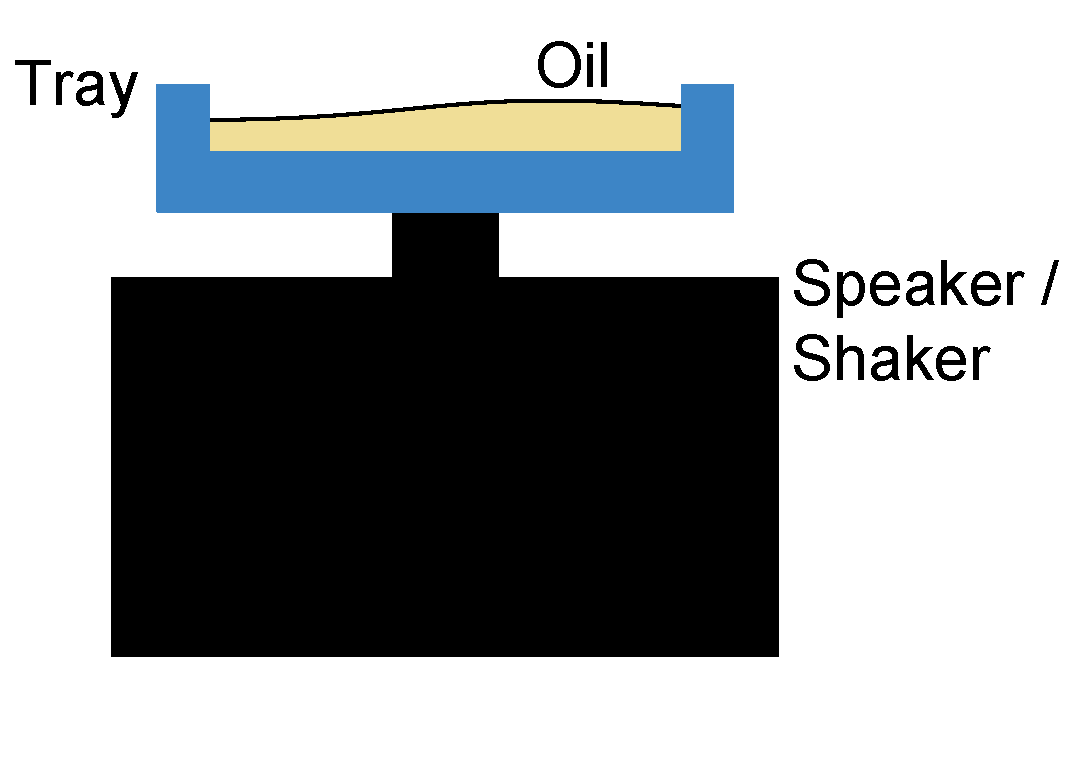
\includegraphics[scale=0.35]{HQASetup.pdf}
	     \caption{The experimental setup. The tray vibrates with an amplitude $A_0$.}
	 \label{regime}
	\end{figure}
	       
	       The oil droplet of diameter $D$ bounces in the regime $\gamma<\gamma_F$, where $\gamma_F$ is the Faraday threshold (at this point, Fraday waves appear). The important experimental limits are outlined in \refTab{approxlimits}. 
	       \begin{table}[htdp] 
\caption[Basic Table 1]{Approximate Limits for Bouncing Drop Behavior} 
\begin{center} 
\begin{tabular}{c c c} 
\toprule 
  Parameter &  Lower Limit & Upper Limit \\
  \midrule
Viscocity $\nu$ (cSt) & 10 & 100 \\ 
Bath Depth $H$ (mm) & 4 & 10 \\
Frequency $f$ (Hz) & 20 & 150 \\
Amplitude $A_0$ (mm) & 0.1 & 1 \\
Drop Diameter $D$ (mm) & 0.6 & 1.0 \\
\bottomrule 
\end{tabular}
\end{center}
\label{approxlimits} 
\end{table}	

For certain parameters, the bouncing drop will behave differently. The vibration number describes ``the relative magnitude of the forcing frequency and the drop's natural oscillation frequency," and is given by:
	       	      
\begin{equation} \label{vibrationnumber}
V_i = \frac{\omega}{2}\sqrt{\frac{\rho D^3}{2\sigma}}
\end{equation}   	       	       
	       	       The natural frequency of the droplet occurs around $V_i = 0.65$, where the droplet can exhibit both walking and bouncing behaviors. Setting up a plot with $V_i$ on the y axis and (dimensionless) ${\gamma}/{g}$ on the x axis can help in showing the behavior of the droplet, shown in \refFig{regime}. 
	    
	    \begin{figure}[h]
	% the options are h = here, t = top, b = bottom, p = page of figures.
	% you can add an exclamation mark to make it try harder, and multiple
	% options if you have an order of preference, e.g.
	% \begin{figure}[h!tbp]
	   
	       \centering
	    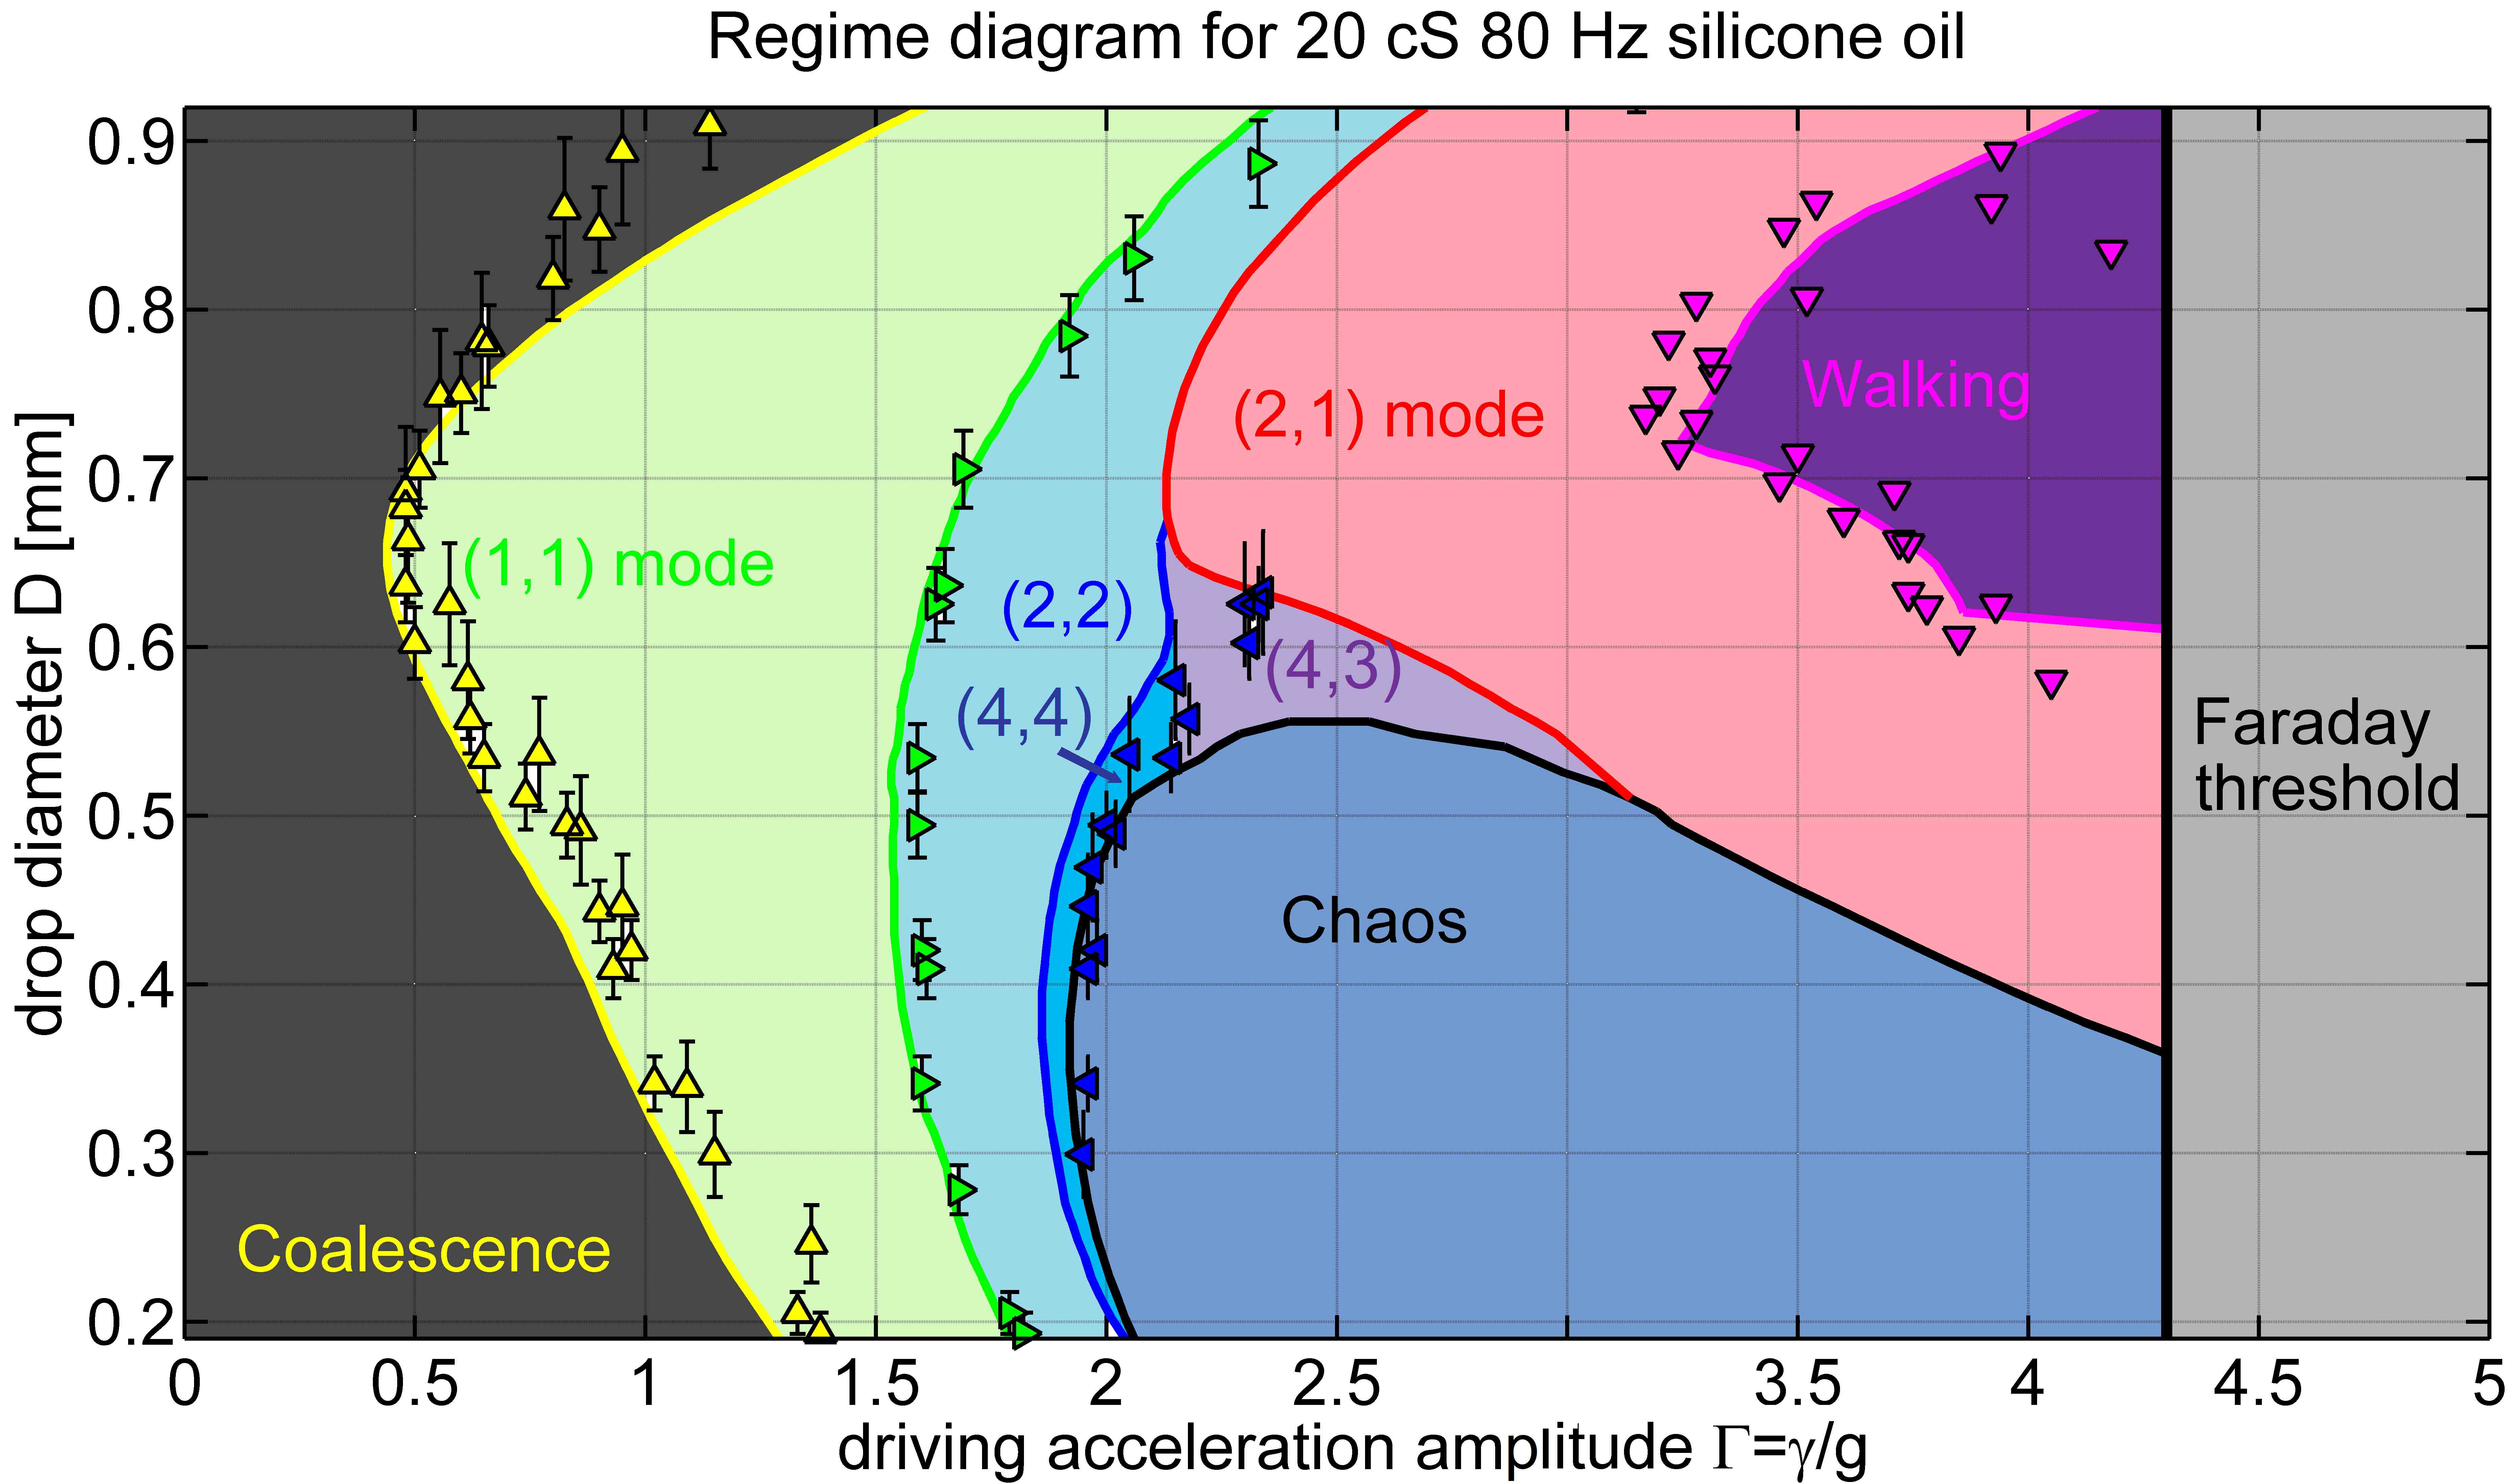
\includegraphics[scale=0.075]{Regime-Mega}
	     \caption{The different bouncing regimes for the oil drops of 20 cS silicon oil and at $f$ = $\omega / 2\pi$ = 80 Hz. The parameters ($m$,$n$) describe the droplet that bounces $n$ times in $m$ forcing periods. }
	 \label{regime}
	\end{figure}

The various modes seen in \refFig{regime} can be described by ($m$,$n$), where $n$ is the number to times the droplet contacts the surface over period $m/f$. For example, in the (1,1) mode, the droplet hits the oil bath once per driving period. In the (2,2) mode, the drop makes two bounces of differing heights. 
	       
            \subsection{Path Memory}
                        
            Path memory is a parameter that can be varied in this setup; it is essentially the damping of the system. Every time the droplet impacts the bath, it creates a radial traveling wave. Over the course of many bounces, a wavefield composed of a superposition of the many waves arises. In this way the wavefield ``remembers" previous interactions. Because droplet motion is influenced by the wavefield, controlling the damping of the wavefield will influence the path of the walker. The heavily damped system has a low memory, while undamped system correspends to higher memory. As one gets closer to the Faraday threshold, one achieves higher and higher memory because waves last for longer. The quantum like features of this experiment arise in the high-memory limit. (For more, Eddi et. al, 2011b: Information stored in Faraday waves.) 

            \subsection{Bound States}
            A bouncing droplet creates a damped wave that depends on the driving acceleration (${\gamma_m}/ g$) CITE: Protiere 2005. A periodic damped wave allows for two bouncers to form a ``bound state".  Starting far away from one another, the two droplets drift towards one another until a fixed distance $d_{0}^{bd}$. Increasing driving acceleration will decrease the value of $d_{0}^{bd}$. These bound bouncers form triangular lattices, and their periodicity is highly sensitive to the mass of the droplet. (LOOK AT EDDI ET ALL 2008).
            
            Walkers can also form bound states. Two walkers of the same size that are approaching one another can form an orbit around their center of mass. Between the two droplets is the fixed distance $d_{n}^{orb}$ given by
            
\begin{equation} \label{orbital}
d_{n}^{orb} = (n - \epsilon_0)\lambda_F
\end{equation}         
where $\epsilon_0$ is a fixed distance which is the same for all orbitals of these walkers (usually in the range $0.15 < \epsilon_0 < 0.25$ depending on droplet diameter), and $n = 1,2,3$... for drops that are in phase or $n = 1/2, 3/2, 5/2$... for drops out of phase. Orbiting periods are approximately porpotional to $d_{n}^{orb}$, which ends up meaning that the velocity of the orbiting walkers is a little less than the velocity of a free walker CITE: Protiere 2006. Orbiting of different sized droplets can also arise.      

            \subsection{Scattering States}
            Two identical walkers headed towards each other can form fixed orbits, or they can scatter. The droplets are deflected through their wavefields (they never actually make contact with one another)            
            \subsection{Single-Particle Diffraction}
In 2006 Couder and Fort showed that the system had properties that were strikinly similar to two famous and controversial quantum experiments (Couder and Fort, 2006). They were able to demonstrate that a single walker travelling through one slit seemed to have its direction altered seemingly randomly, before continuing forward on its new path. By statistically analyzing many trials, Couder and Fort showed that the histogram of the ``diffraction" actually resulted in a diffraction pattern strikingly similar to the single photon diffraction experiment performed by Taylor in 1909. 

Next, Couder and Fort added a second slit next to the first one. Now a single walker could pass through  one of two slits, and it was discovered that a histomgram of this data returned another diffraction pattern. This result is of course reminiscent of one of the most famous experiments in physics: Young's double slit diffraction with photons and electrons. 
    
Using a numerical simulation, Couder and Fort were able to reproduce similar results. 
    
As Couder and Fort mention in their paper: ``A discussion of the relation between these single-particle experiments and those concerning elementary particles is unavoidable." Important differences and similarities are then described between the quantum system and the quantum-like system. For the differences: we have a dissapative system, where energy is continually put in through the vibration of the tray; the particle can be followed;\footnote{C and F note that it'd be impossible to dectect the particle without disturbing it "by any means at its scale," like a bouy, for example. As the bouy floated it would interfere with the system by altering the wave pattern on the surface.} it's really effectively moving in two dimensions; the velocity is measurable; and the probability distributuion is linked with the wave amplitude (rather than it's intensity). And then of course, the similarities: an uncertainty priciple arises from the statistical data (and without knowledge of the actual paths followed by the walkers); and some others that were unclear...

Recently, Harris attempted to reproduce single slit interference. With better technology, new results were found. Using a looping guiding batt, trajectories were found to follow the same loop without deviating. Only at a very high memory were there chaotic paths.
	       \subsection{Tunneling}
	       The guiding wave field can be partially reflected off of an edge or even a change in depth of the oil bath. This effect can be seen when a walker is pushed back from a under-the-surface step, seemingly without any contact. In rare cases, the walker will actually tunnel across the step; that is, it will continue to walk along the surface of the oil bath and pass over the step without reflection. In the first experiment done by Eddi et al., they demonstrated tunneling by by building square ``corrals" of varying thicknesses. In the second experiment, they built a rhombus shape which forced the walker across the center of a rhombus. The barrier was placed perpendicular to the direction of travel of the walker, so that it would hit the wall directly rather than at an angle (as in the square corral). ``The tunneling probability decreases exponentially with the barrier width and increases as the Faraday threshold is approached." Eddi et. al also found that the probability of tunneling increased with the velocity of the walker. (For more, Eddi et. al 2009b: Unpredictable Tunneling of a classical wave-particle association.)
	       
	       
	        The unpredictability of the tunneling comes from the complex interatction between the drop and its guiding wave. 

\subsection{Motion in a Confined Geormetry}
By tracking the droplet as it bounces around the tray over a period of time, one can look at the overall statistical behavior of the droplet. Two experiments tracked walkers in an experimental coral (Harris and Bush, 2013, Harris et al. 2013) in the high-memory, chaotic motion regime. A histogram of the statistical data shows that the "probability of finding a walker at a given point in the corral is roughly prescribed by the amplitude of the Faraday wave mode of the cavity at the prescribed forcing frequency."

Quantum corral experiments performed by Crommie et al. (Crommie et al. 1993 a b) present similar findings. In the experiment, electrons were confined in a Cu(III) substrate using barriers of iron adatoms. Using tunneling spectroscopy, the electrons were found to have a specific resonances depending on the corral shape. As in the case of Harris' circular corral experiment where the corral and the Faraday wavelength, $\lambda_F$, dictate the wavelike statistical patter, in the quantum experiment the corral and the \textit{de Broglie} wavelength, $\lambda_{dB}$, dictate the form of the wavelike statistical pattern. 

\subsection{Walker Trajectories}
In the regime of walkers we have $R_e \sim 20$, $B_0 \sim 0.1$, and $W_e \sim 0.1$. For the millimeric walkers, the dominant force comes from impact of the curvature of the surface. Gilet and Bush (2009: Chaotic bouncing of a drop on a soap film, and the fluid trampline: droplets bouncing on a soap film) show that the surface of the vibrating oil can be modeled with a soap film, where the soap film acts like a linear spring. 

As the oil bath is forced up and down, a tiny droplet of oil will ``walk" across the surface. Mol\'{a}\v{c}ek and Bush have developed an equation of a droplet that describes the trajectory of the walking droplet, ignoring the verical dynamics by time averaging them out (cite: J. Mol\'{a}\v{c}ek and J. W. M. Bush, ``Drops walking on a vibrating bath: towards a hydrodynamic pilot-wave theory" J. FluidMech. 727, 612-647 (2013).). The trajectory of the walking droplet of mass $m$ at position $\textbf{x}(t) = (x(t),y(t))$ is given by
\begin{equation}
m \ddot{\textbf{x}} + D \dot{\textbf{x}} = -mg\nabla h(\textbf{x},t) 
\end{equation}
where $D$ describes the drag coefficient and $h(\textbf{x},t)$ describes the shape of the wavefield. Thus the second term describes the time averaged drag from both the flight and the impact of the droplet (as usual, depends on the velocity), and the third term describes the propulsive wave force resulting from drops landing on the inclined wave surface. 

The wavefield is quite complicated because it depends on the memory. For a single impact of a droplet, Oza et al. argue the surface wave can be approximated with an integral of a monochromatic radial Bessel function of the first kind

\begin{equation}
h(\textbf{x},t) = \frac{F}{T_F} \int_{-\infty}^{t} J_0 \frac{(k_F |\textbf{x}(t)-\textbf{x}(s)|)}{|\textbf{x}(t)-\textbf{x}(s)|} (\textbf{x}(t)-\textbf{x}(s))e^{-(t-s)/(T_F M_e)} ds
\end{equation}
with $F$ giving the wave force coefficient (estimated in the above source), $T_F$ describing the Faraday period, and $k_F$ describing the Faraday wave number determined by the Faraday wavelength $\lambda_F = 2π/k_F$ (integral from A. U. Oza, D. M. Harris, R. R. Rosales, and J. W. M. Bush, "Pilot-wave dynamics in a rotating frame: on the emergence of orbital quantization" J. Fluid Mech. 744, 404-429 (2014).). (Faraday was a popular guy.) Finally, that last term $M_e$ is the nondimensional memory parameter $M_e = T_d/[T_F(1-\gamma / \gamma_F)]$ (with $T_d$ being the unforced decay time).

\section{Experimental Setup}

\section{Bohmian Mechanics}

\subsection{Formalism}
\subsubsection{The Schroedinger Equation and $\psi$}

We begin with the Schoedinger equation

\begin{equation}
i \hbar \frac{\partial}{\partial t}\psi = \hat H \psi
\end{equation}
where $\hat H$ is the Hamiltonian and $\psi$ is the wavefunction. The Hamiltonian can be expanded (assuming there is no electric field) to give

\begin{equation}
\label{SE}
i\hbar\frac{\partial}{\partial t} \psi(\mathbf{x},t) = \left [ \frac{-\hbar^2}{2 m}\nabla^2 + V(\mathbf{x},t)\right ] \psi(\mathbf{x},t)
\end{equation}
where $V(\mathbf{x},t)$ is the potential energy of the system. The solution $\psi$ is of the form:

\begin{equation}
\psi(\mathbf{x},t) = R(\mathbf{x},t) e^{i S(\mathbf{x},t) / \hbar}
\end{equation}
where $S$ and $R$ are real. Plugging in our equation for $\psi$ into the Schoedinger equation (\refeq{SE}) will produce two separate equations: one giving the time derivative of $R$ and the second giving the time derivative of $S$. From these equations, a Hamilton-Jacobi equation can be written for a quantum system.
    Let's begin by computing the left hand side of \refeq{SE} in terms of $R$ and $S$.   

$$
\begin{align*}
i\hbar\frac{\partial}{\partial t} \psi(\mathbf{x},t) &= i \hbar\left(\frac{\partial R}{\partial t} e^{i S / \hbar} + R \frac{i}{\hbar}\frac{\partial S}{\partial t} e^{i S / \hbar}\right)
\\ &= i \hbar \left(\frac{1}{R} \frac{\partial R}{\partial t} + \frac{i}{\hbar}\frac{\partial S}{\partial t}\right) \psi(\mathbf{x},t) 
\\ &= \left(i \hbar \frac{1}{R} \frac{\partial R}{\partial t} - \frac{\partial S}{\partial t}\right) \psi(\mathbf{x},t)
\end{align*}
$$
Let's leave that alone for a little bit, while we focus on the right hand side of \refeq{SE}. Since it's a little more complicated, we will start with one term of the right hand side:

$$
\begin{align*}
\nabla^2 \psi(\mathbf{x},t)  &= e^{i S / \hbar} \nabla^2 R + \left(\frac{i}{\hbar}\right)^2 (\nabla S)^2 R e^{i S / \hbar} + \left(\frac{i}{\hbar}\right) R e^{i S / \hbar} (\nabla^2 S) + \left(\frac{2i}{\hbar}\right) (\nabla R \cdot \nabla S) R e^{i S / \hbar}
\\ &= \left(\frac{\nabla^2 R}{R} - \left(\frac{\nabla S}{\hbar}\right)^2  + \left(\frac{i \nabla^2 S}{\hbar}\right) + 2 i \left(\frac{\nabla R \cdot \nabla S}{\hbar}\right) \right) \psi(\mathbf{x},t) 
\end{align*}
$$

Now the hard part is done, and we can say that the right hand side of \refeq{SE} is given by 

$$
\begin{align*} 
\left [ \frac{-\hbar^2}{2 m}\nabla^2 + V(\mathbf{x},t)\right ]\psi(\mathbf{x},t) &= \left [-\frac{\hbar^2  \nabla^2 R}{2 m R} + \left(\frac{(\nabla S)^2}{2 m}\right)  - i \hbar \left(\frac{\nabla^2 S}{2 m}\right) - i \hbar \left(\frac{\nabla R \cdot \nabla S}{m}\right) + V(\mathbf{x},t) \right]\psi(\mathbf{x},t) 
\end{align*}
$$

Ok, now that we've got that done, the next part will be super easy. Starting with Schrodinger's equation and plugging in left and right hand sides we calulated seperately. 

$$
i\hbar\frac{\partial}{\partial t} \psi(\mathbf{x},t) = \left [ \frac{-\hbar^2}{2 m}\nabla^2 + V(\mathbf{x},t)\right ] \psi(\mathbf{x},t)
$$
$$
\left(i \hbar \frac{1}{R} \frac{\partial R}{\partial t} - \frac{\partial S}{\partial t}\right) \psi(\mathbf{x},t) =\left [-\frac{\hbar^2  \nabla^2 R}{2 m R} + \left(\frac{(\nabla S)^2}{2 m}\right)  - i \hbar \left(\frac{\nabla^2 S}{2 m}\right) - i \hbar \left(\frac{\nabla R \cdot \nabla S}{m}\right) + V(\mathbf{x},t) \right]\psi(\mathbf{x},t) 
$$
Now we can divide out $\psi$ from both sides
$$ 
i \hbar \frac{1}{R} \frac{\partial R}{\partial t} - \frac{\partial S}{\partial t} = -\frac{\hbar^2  \nabla^2 R}{2 m R} + \left(\frac{(\nabla S)^2}{2 m}\right)  - i \hbar \left(\frac{\nabla^2 S}{2 m}\right) - i \hbar \left(\frac{\nabla R \cdot \nabla S}{m}\right) + V(\mathbf{x},t)
$$
and group the imaginary numbers on the left side and the real numbers on the right side 
$$ i \hbar \frac{1}{R} \frac{\partial R}{\partial t} + i \hbar \left(\frac{\nabla^2 S}{2 m}\right) + i \hbar \left(\frac{\nabla R \cdot \nabla S}{m}\right) = \frac{\partial S}{\partial t} -\frac{\hbar^2  \nabla^2 R}{2 m R} + \left(\frac{(\nabla S)^2}{2 m}\right)  + V(\mathbf{x},t)
$$
Recall that both $S$ and $R$ are real. Note that the only way for all of the imaginary terms to equal all of the real terms is if they both equaled zero.
$$i \hbar \left(\frac{1}{R} \frac{\partial R}{\partial t} + \frac{\nabla^2 S}{2 m} + \frac{\nabla R \cdot \nabla S}{m}\right) = \left(\frac{\partial S}{\partial t} -\frac{\hbar^2}{2m}\frac{\nabla^2 R}{R} + \frac{(\nabla S)^2}{2 m}  + V(\mathbf{x},t) \right) = 0
$$
This then gives us two sepeate equations, one for the time derivative of $R$ and another for the time derivative of $S$.

\begin{equation}
\label{dR/dt}
\frac{\partial R}{\partial t} = -\frac{R}{2 m}\left(\frac{\nabla^2 S}{m}-2\nabla R \cdot \nabla S\right)
\end{equation}


\begin{equation}
\label{dS/dt}
\frac{\partial S}{\partial t} = \frac{\hbar^2}{2m}\frac{\nabla^2 R}{R} - \frac{(\nabla S)^2}{2 m} - V(\mathbf{x},t)
\end{equation}

What does this do for us? Both equations will provide helpful descriptions of our system.

\subsubsection{The Quantum Potential}

We can rewrite \refeq{dS/dt} in a provokative way 

\begin{equation}
\label{BohmHamiltonian}
- \frac{\partial S}{\partial t} = \frac{(\nabla S)^2}{2 m} + V(\mathbf{x},t) + \frac{\hbar^2}{2m}\frac{\nabla^2 R}{R}
\end{equation}
which should look suspiciously familiar. If I were to tell you that $\nabla S$ had units of momentum and $\partial S/\partial t$ units of energy, then this equation would look a lot like a Hamiltonian! The first term takes care of the kinetic energy, the second is the potential energy term, but we have this mysterious third term which we haven't ever encountered in classical mechanics. If we define this term as our ''quantum potential" 

\begin{equation}
\label{QuantumPotential}
U(\mathbf{x}) =  \frac{\hbar^2}{2m}\frac{\nabla^2 R}{R} = \frac{\hbar^2}{4m}\left[\frac{1}{2} \frac{\nabla^2 P}{P} - \frac{(\nabla P)^2}{P^2}\right] 
\end{equation}
then we really \textit{can} think of \refeq{BohmHamiltonian} as a Hamiltonian with an extra potential term thrown in to make it "quantum." Note that in cases where $\hbar$ is much smaller than the rest of the terms (i.e. not the quantum realm), then this quantum potential term goes away, and we are left with the regular Hamilton equation from classical mechanics. 

Recall that when writing a Hamiltonian, the potential terms govern the forces on the particle. For a conservative system, the force is given by F(x) = -$\partial U/\partial x$. If we include a quantum mechanical potential in our Hamiltonian, then this potential must cause a force on the paticle in addition to the one supplied by the $V(x)$ term. 


\subsubsection{Continuity Equation}
Plugging in the probability density $P(\mathbf{x},t) = R^2(\mathbf{x},t)$ into \refeq{dR/dt} also gives us something quite interesting.

MATH?

which we can finally express as 

\begin{equation}
\label{ProbCurrent}
\frac{\partial P}{\partial t} + \nabla \cdot \left( P \frac{\nabla S}{m} \right)
\end{equation}

In describing the quantum potential term it was mentioned that $\nabla S$ can be thought of as momentum, so then from our classical relationship between momentum and velocity  $\textbf{v}(\textbf{x},t)=\nabla S/m$ can be thought of as velocity. Then by defining the probability current as $j(\mathbf{x},t) = P\nabla S/m$ then we recover

\begin{equation}
\label{ProbCurrent}
\frac{\partial P}{\partial t} + \nabla \cdot j(\mathbf{x},t)
\end{equation}
known as the continuity equation! This tells us that $P$ is conserved over time.

\subsubsection{Finding $R$ and $S$}



	\chapter{Introduction to Tunneling in QM}	


\section{Wavefunction}	
In classical mechanics, one can describe a particle with six variables: three position indicators ($x$, $y$, $z$), and three momentum indicators ($p_x$, $p_y$, $p_z$). One can find a function to represent variable by making multiple measurements across time, and discover an expression $x(t)$ that describes the particles location in space along the x dimension at time $t$. When all six variables can be described by a function, one can describe the position of the particle at any time.  

In quantum mechanics however, Heisenberg's uncertainty priciple limits the knowledge of position and momentum: 
$$\sigma_{x} \sigma_{p} \geq \hbar/2. $$
This equation states that as one knows more about the position of the system, then one loses knowledge about the momentum of the system, and vis versa. It's a tradeoff inherent to the nature of the system, not due to experimental deficiences. And it means that the strategy of finding equations for position and momentum of a system are no longer possible. If a particle has no exact position, can one represent where it might be? One can use a wave describing the probability of finding the particle at that position. The square root of this wave is called the wavefunction, and is represented by $\Psi(x, t)$.


\section{Schroedinger's Equation}

The wavefunction $\Psi(x, t)$ is goverened by the Schroedinger equation:

$$i\hbar\frac{\partial}{\partial t} \Psi(x,t) = \left [ \frac{-\hbar^2}{2m}\frac{\partial^2}{\partial x^2} + V(x,t)\right ] \Psi(x,t) $$
where $V(x,t)$ is the given potential, $m$ is the mass of the particle, and $\hbar$ is the reduced Planck's constant. For potentials that do not change in time, one can use separation of variables to arrive at the time-independant Schroedinger equation
$$E \Psi(x,t) = \left [ \frac{-\hbar^2}{2m}\frac{\partial^2}{\partial x^2} + V(x)\right ] \Psi(x,t)$$
where $E$ is the total energy. The goal is to find $\Psi(x,t)$ knowing the potential $V(x)$.




\section{Barrier Potential}

\section{Energies}
    \subsection{$E = V_0$}
    \subsection{$E > V_0$}
    \subsection{$E < V_0$}
    
    
    
    
\section{Physics}

Many of the symbols you will need can be found on the math page (\url{http://web.reed.edu/cis/help/latex/math.html}) and the Comprehensive \LaTeX\ Symbol Guide (enclosed in this template download).  You may wish to create custom commands for commonly used symbols, phrases or equations, as described in Chapter \ref{commands}.


	\chapter{Experimental Design}

In the our bouncing droplet system we observe surface waves guiding a droplet, and we're interested in learning more about the droplet-wave system in different settings. In this experiment, we will look at how features \textit{underneath} the surface of the oil (i.e. on the ``floor" of the tray) affect the motion of the droplet. 

A raised object on the floor of the tray (but still underneath the surface of the oil) can have an effect on height of the surface waves, and thus, on the motion of the walker. Sometimes a droplet headed towards a raised object will be reflected backwards, as if from a collision with the object. For this reason, we refer to a raised object as a barrier. Oftentimes however, the droplet continues on and crosses the barrier without a collision, this is analagous to ``transmission" the quantum mechanical process of tunneling. In other words, for a given barrier we will see a probability of tunneling unique to that barrier. Other studies have shown that increasing barrier width decreases probability of tunneling\rf{tunneling}. This study looks at how height of the barrier affects the tunneling probability. 

To test the effect of a barrier's height on the probability of tunneling, I used a combination of procedures from the investigations of Bush\rf{pilot-wave}, Couder\rf{Couder2005}, and specifically, Eddi et al.\rf{tunneling}. These were slightly modified to fit some of the unique features of my experiment. In this section I aim to give some of the reasoning behind the tray design and data collection techniques, both of which are not well described in the literature.

\section{Setup}
    The combined setup is shown in \refFig{setup}. A waveform generator creates a sinusoidal signal which is amplified and fed into a shaker. The shaker vibrates the tray vertically. Both the frequency and the amplitude of the vertical oscillations can be controlled. 
    
    An accelerometer records the vertical acceleration of the tray and is read by an oscilloscope. A camera records the droplet as it bounces along the surface of the oil.  
    
\begin{figure}[h!]
	\centering
	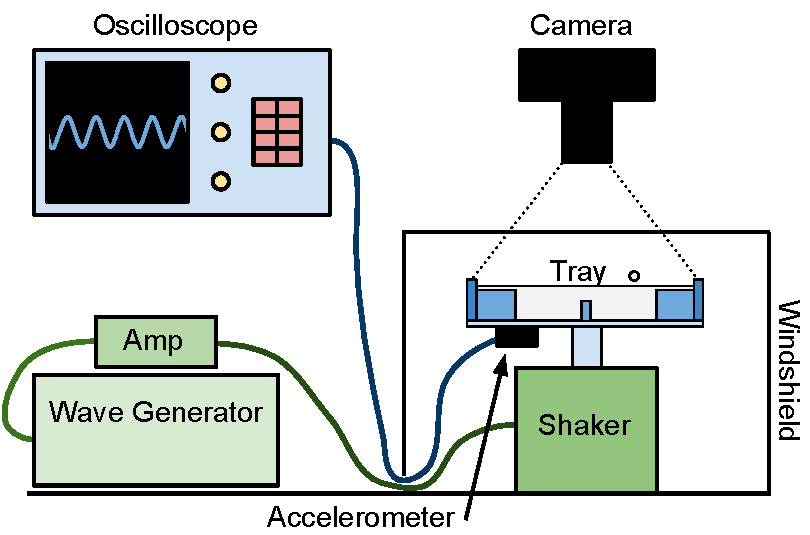
\includegraphics[scale=0.8]{Setup.pdf}
	\caption{The experimental setup. The amplified signal from the wave generator drives the shaker. The accelerometer generates a signal which is read by the oscilloscope. The shield blocks disturbances to the experiment, while allowing the camera to document the trials.}
	\label{setup}
\end{figure}

\section{Materials}
The key components of this experiment are the shaker, the oil, and the tray. In this section I'll describe the specifics of the holy trinity, as well as some of the additional components used in data collection. 

\subsection{Tray}
The tray was made of plastic parts machined by the (MODEL NUMBER?) laser cutter. They were then glued together with GLUE?. The tray's design, which was based off of the tray in the tunneling experiment done by Eddi et al.\rf{tunneling}, naturally guides the droplet into a perpendicular collision with the barrier. The tray schematic is shown in \refFig{tray}. 

\begin{figure}[h!]
	\centering
	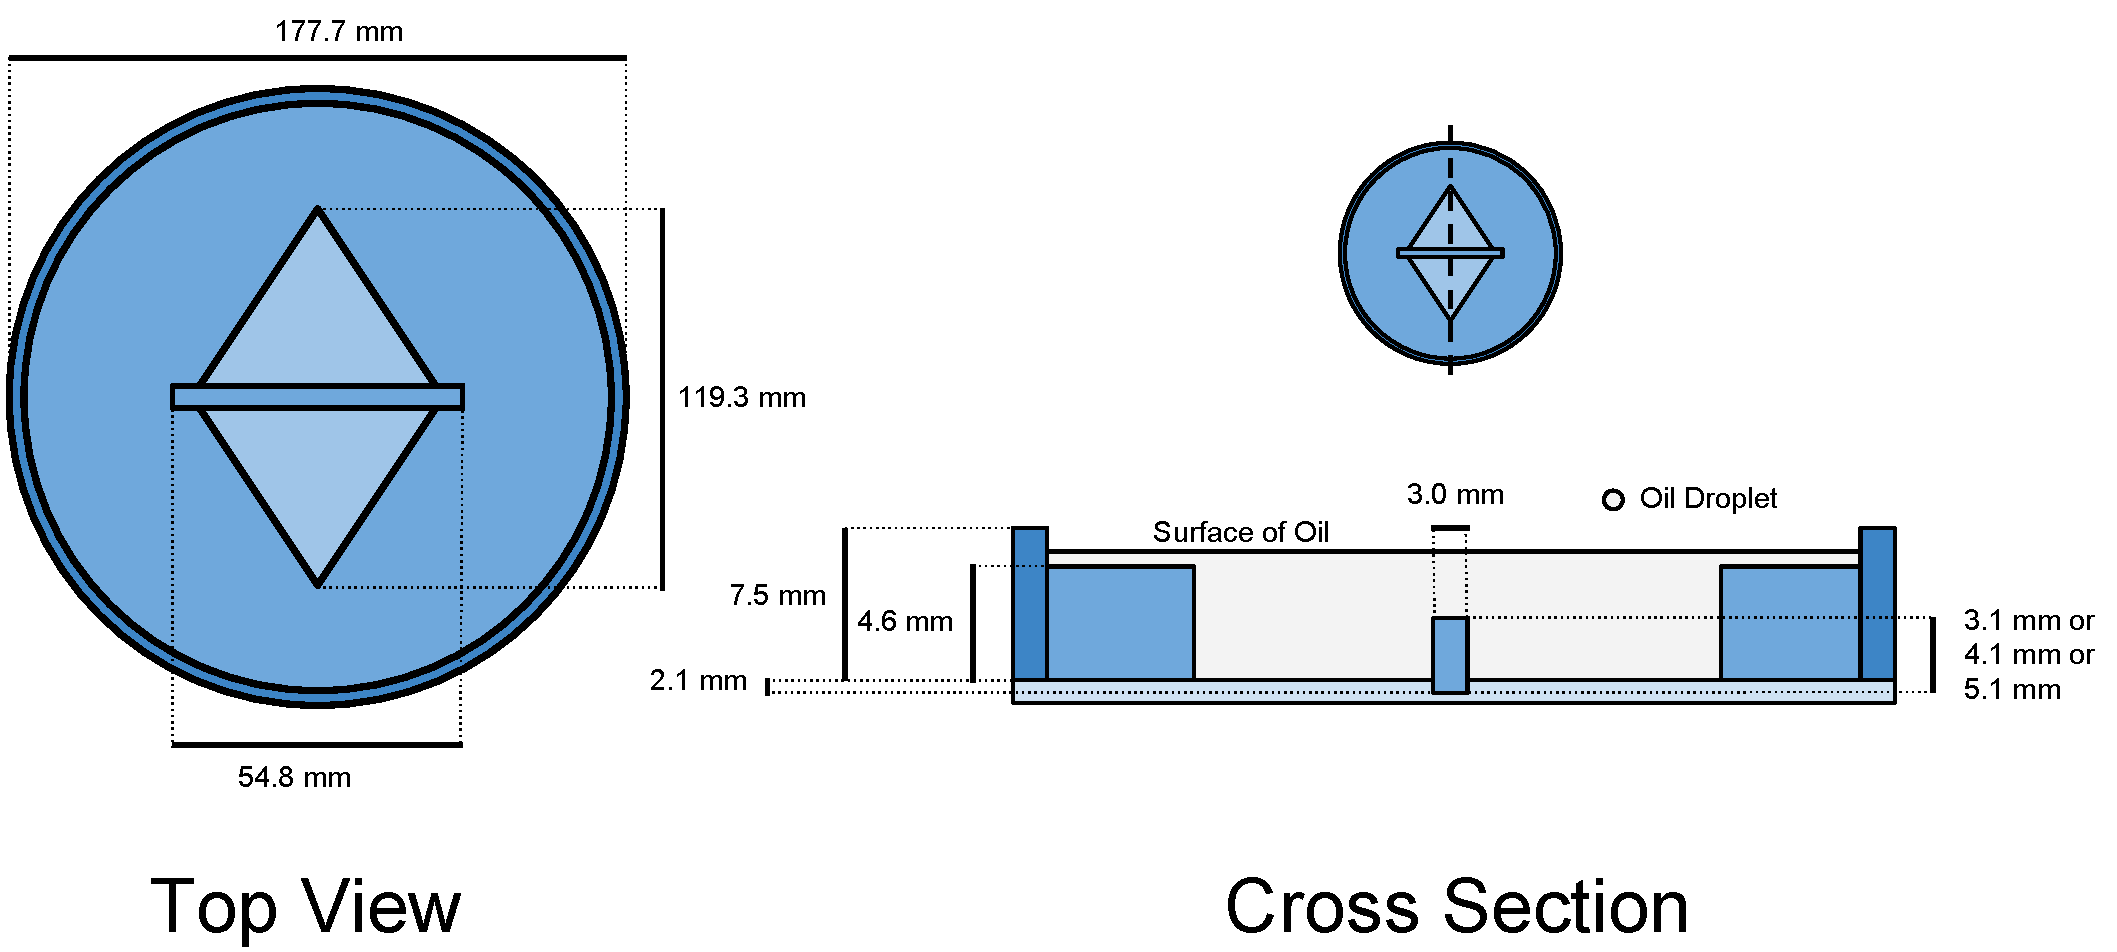
\includegraphics[scale=0.48]{Tray.pdf}
	\caption{The specifications of the tray design. The top view (left) highlights the main elements in the tray, while the cross section (right) illustrates the topography of the tray. Height is represented by the shading; darker shading is higher.}
	\label{tray}
\end{figure}

A thin layer of oil spills over the constraining rhombus shape. As long as the layer is thin enough, the droplet will remain in the rhombus container, but the waves will continue to propagate unimpeded. This gives the waves time to decay, and means that the droplets motion isn't chaotically affected by reflections of previous waves from the sidewalls, and is instead guided only by the unreflected waves. 

The rhombus shape serves to steer the droplet into a perpendicular collision with the barrier. This works because the droplet will pin-ball its way into the acute corner of the rhombus, and will shoot out in a straight line, directly towards the barrier.  (FIGURE of pinballing droplet?)

I designed my experiment to test barriers of three different heights: $2.75~\mathrm{mm}$, $3.0~\mathrm{mm}$, and $3.25~\mathrm{mm}$, measured from the bottom of the rhombus. A thin barrier of plastic made by the laser cutter has the tendency to bend and warp over time. The solution to this problem was to make these barriers taller than the specified heights, and create an cut-out in the rhombus so they could be inserted. The barrier cut-outs were deep enough to exactly counter the added height of the barrier, so the barriers still had (when measured from the surface of the rhombus) heights of $2.75~\mathrm{mm}$, $3.0~\mathrm{mm}$, and $3.25~\mathrm{mm}$. This also solved the problem of fixing the barriers in place, but still making them easily removable. These heights were chosen because they allowed for both passage over and blockage by the barriers. At the lowest heights, most droplets crossed over, whereas for taller barriers most droplets were blocked. 


The bottom of the tray was painted black in order to improve contrast, allowing the droplet to be more easily tracked by eye and by camera.

\subsection{Silicon Oil}
    Silicon oil is the ideal choice of fluid for this experiment because it remains clean, it doesn't evaporate, and it can be purchased at specific viscosities. The silicone oil used in this experiment had a viscosity of 20 cSt (its viscosity is a little closer to water than olive oil) and was purchased from Clearco Products Co. Inc., Bensalem PA (CAS No: 63148-62-9). 20 cSt silicone oil, like the one used by Bush et al.\rf{pilot-wave} was chosen because it gives a larger walking regime\rf{pilot-wave} than more viscous oil, such as the 50 cSt viscosity oil used by Couder\rf{Protiere2005}. The tray requires about $20~\mathrm{mL}$ of fluid.
    
    It is of vital importance to keep the oil as clean as possible because it keeps the droplet bouncing for longer. This means protecting from particulate matter that is already in the tray. Contamination can be minimized by cleaning the tray before pouring the oil in.
    
\subsection{Shaker}
    To shake the tray, we used a mechanical wave driver made by Pasco Scientific, Roseville CA, model SF-9324. This shaker was designed to drive a string or an elastic cord, not a $200$ gram tray with oil inside, which was probably at the limit of what the shaker can handle. 

\subsection{Waveform Generator and Amplifier}
    The shaker was driven with the Agilent Arbitrary Waveform Generator model 33210, which was controlled digitally and thus created consistent waves.  
       
    Adding a Lepai LP2020A+ digital amplifier to the wavefunction generator meant the amplitude of the tray could be precisely controlled. This signal was then fed into the shaker.    
            
\subsection{Accelerometer}  
    Knowing the tray's acceleration allows us to characterize the behavior of our system. To measure acceleration, we attached an ADLX 326 triple axis accelerometer (made by Adafruit, New York City NY) to the bottom of the tray. The method of attachment was screws, since it provided a much more firm hold than tape or glue while allowing for removal. The accelerometer has a range of $\pm$16$g$, perfect for measuring the accelerations in our setup, usually below $5g$'s. 
      
      The signal from the z-axis of the accelerometer was output directly into the oscilloscope. For the vibrating tray, the output was approximately sinusoidal (as expected). The spec sheet for the accelerometer indicates that the sensitivity can be translated to $57 \pm 6~\mathrm{mV/g}$. 
 
    
\subsection{Shield}
    A large, see-through cylinder (covered at one end) was manufactured using the laser cutter. When placed over the tray, it served the purpose of keeping the oil clean from particulate matter and preventing wind currents from influencing the motion of the walker.       
   
\subsection{Leveling Platform}
    A leveling platform was made out of wood supports the shaker. Three adjusters allowed for precise adjustment of tilt. The tray was tuned using a level placed inside the tray (before the oil was added). 

\subsection{Camera}       
 
To document trials, a Sony RX100 camera supported by a tripod aimed directly down at the tray. 

\section{Procedure}
Once the exact walking parameters are established (frequency and driving amplitude), tunneling measurements and a few different barrier heights can be made. 

\subsection{Finding the Walking Regime}

Before investigating the rate of tunneling using different barriers, a rough estimate of the walking regime at a frequency of $80~\mathrm{Hz}$ must be made. A ``map" similar to the one in \refFig{regime} will be sketched out, but rather than looking at all of the different kinds of bouncing we will limit ourselves to only the walking regime. Reproducing this figure allows us to find the parameters that are specific to our unique setup, which could have slightly different height, tray, oil, and shaker configurations than those used in the literature. 

Droplet size is measured using a recorded video of the walking droplet in motion. By comparing the number of pixels making up the diameter of the droplet (unknown measurement) to the number of pixels making up the diameter of the tray (known measurement), we can estimate the length associated with  each pixel, and thus find the diameter of the droplet in centimeters. 

Driving acceleration values are measured by the accelerometer and displayed on the oscilloscope. 

To ensure that every trial has the same oil depth, we must measure the volume of the oil before filling the tray. Knowing the volume of the tray and of each barrier, we can get a value for the oil depth without interfering with the system. In this way, oil height can be kept constant.

\subsection{The Experiment}

Tunneling was examined for three different barrier heights. At each height (and at a constant frequency of 80 Hz and constant driving acceleration), a string of continuous collisions were filmed with the camera. From this data, a basic tunneling probability was calculated, which provides the most simplistic analysis of this system. 

The tray is designed such that most of the droplet's collisions with the barrier occur ``head on" (i.e. perpendicular to the length of the barrier), but not all collisions unfold ideally. A more involved analysis in \textit{Tracker} requires looking at the component of velocity of the droplet perpendicular to the length of the barrier, and determining the probability of tunneling given this value. Since not all collisions in the simplistic analysis occur at the same velocity, this method allows for a more methodical analysis of the phenomena. 


	\chapter*{Conclusion}
         \addcontentsline{toc}{chapter}{Conclusion}
	\chaptermark{Conclusion}
	\markboth{Conclusion}{Conclusion}
	\setcounter{chapter}{4}
	\setcounter{section}{0}
	
%Here's a conclusion, demonstrating the use of all that manual incrementing and table of contents adding that has to happen if you use the starred form of the chapter command. The deal is, the chapter command in \LaTeX\ does a lot of things: it increments the chapter counter, it resets the section counter to zero, it puts the name of the chapter into the table of contents and the running headers, and probably some other stuff. 

%So, if you remove all that stuff because you don't like it to say ``Chapter 4: Conclusion'', then you have to manually add all the things \LaTeX\ would normally do for you. Maybe someday we'll write a new chapter macro that doesn't add ``Chapter X'' to the beginning of every chapter title.

The question we sought to answer was: how does tunneling probability change with the value $h$ of oil above the barrier? Our results showed that tunneling is highly sensitive in this system, and even changes in height on the order of fractions of a millimeter are enough to radically influence the proportion of tunneling droplets. Using a barrier of width $e~=~3.0~\mathrm{mm}$, it was found that a value of $h~=~1.0~\mathrm{mm}$ produced tunneling in every interaction, while for a value of $h~=~1.5~\mathrm{mm}$ there was no tunneling. In between this range was a sweet spot of $h~=~1.25~\mathrm{mm}$ where tunneling appeared probabilistic, but still somewhat dependent upon droplet diameter and droplet velocity. It would appear that for a given barrier, a droplet with a higher momentum is more likely to tunnel than a droplet with lower momentum.


The main limitations in this investigation had to do with consistency of parameters between trials, and dearth of data points. A better shaker would have significantly improved these things. The damping of the shaker we used made keeping a the same memory in every trial difficult, and limited the number trials and interactions that were filmed. The one modeled in \rf{shaker}, shakes the whole tray at the same time and with same amplitude for hours. These shakers of course, cost more than the budget allowed for, but a even conducting the tests suggested in the paper would have allowed for diagnosis of these issues. Another difficulty was in measuring the height of the oil within a trial. When removing each barrier, a certain amount of oil was lost. While this value was estimated, it still was a source of uncertainty and it introduced contamination from the pliers to get into the oil. Additionally, surely there exists a better way to measure oil depth than computing the volume of space inside the tray, but a cheap alternative was not discovered. This would have also increased uncertainty in the measurements of $h$. Using barriers of height $2.90~\mathrm{mm}$ or $3.10~\mathrm{mm}$ would have allowed for greater definition in the range of tunneling heights in \refFig{tbh}.


A few words of advice for those seeking to recreate the experiment: take your time in setting up the device, ensuring that the tray is level and that it vibrates vertically. Invest in good silicone oil, and do your best to limit any contamination of the oil. Finally, there is an accelerometer out there that does what you need it to, your task is simply to find it. 

%If you feel it necessary to include an appendix, it goes here.
	\appendix

	\chapter{The First Appendix}
An appendix full of awesome
	\chapter{The Second Appendix, for Fun}
An appendix full of win


%This is where endnotes are supposed to go, if you have them.
%I have no idea how endnotes work with LaTeX.

  \backmatter % backmatter makes the index and bibliography appear properly in the t.o.c...

% if you're using bibtex, the next line forces every entry in the bibtex file to be included
% in your bibliography, regardless of whether or not you've cited it in the thesis.
  \nocite{*}

% Rename my bibliography to be called "Works Cited" and not "References" or ``Bibliography''
% \renewcommand{\bibname}{Works Cited}

%    \bibliographystyle{bsts/mla-good} % there are a variety of styles available; 
%  \bibliographystyle{plainnat}
% replace ``plainnat'' with the style of choice. You can refer to files in the bsts or APA 
% subfolder, e.g. 
 \bibliographystyle{APA/apa-good}  % or
 \bibliography{thesis}
 % Comment the above two lines and uncomment the next line to use biblatex-chicago.
 %\printbibliography[heading=bibintoc]

% Finally, an index would go here... but it is also optional.
\end{document}
